\INEchaptercarta{Caracterización educativa de los faltantes}{}



\cajita{Faltas judicales}{El número de faltas judiciales tiene una tendencia ascendente. Para el año 2014 se registraron 23,564 las cuales, respecto al año anterior, representan un aumento en un 6.9\%.}{Número de faltas judiciales}{República de Guatemala, serie histórica, en datos absolutos}{\ \\[0mm]\begin{tikzpicture}[x=1pt,y=1pt]  % Created by tikzDevice version 0.10.1 on 2016-02-29 15:06:30
% !TEX encoding = UTF-8 Unicode
\definecolor{fillColor}{RGB}{255,255,255}
\path[use as bounding box,fill=fillColor,fill opacity=0.00] (0,0) rectangle (289.08,198.74);
\begin{scope}
\path[clip] (  0.00,  0.00) rectangle (289.08,198.74);

\path[] (  0.00,  0.00) rectangle (289.08,198.74);
\end{scope}
\begin{scope}
\path[clip] (  0.00,  0.00) rectangle (289.08,198.74);

\path[] ( 12.62, 15.61) rectangle (280.54,191.48);

\path[] ( 12.62, 40.20) --
	(280.54, 40.20);

\path[] ( 12.62, 74.22) --
	(280.54, 74.22);

\path[] ( 12.62,108.23) --
	(280.54,108.23);

\path[] ( 12.62,142.24) --
	(280.54,142.24);

\path[] ( 12.62,176.25) --
	(280.54,176.25);

\path[] ( 12.62, 23.20) --
	(280.54, 23.20);

\path[] ( 12.62, 57.21) --
	(280.54, 57.21);

\path[] ( 12.62, 91.22) --
	(280.54, 91.22);

\path[] ( 12.62,125.23) --
	(280.54,125.23);

\path[] ( 12.62,159.25) --
	(280.54,159.25);

\path[] ( 43.53, 15.61) --
	( 43.53,191.48);

\path[] ( 95.06, 15.61) --
	( 95.06,191.48);

\path[] (146.58, 15.61) --
	(146.58,191.48);

\path[] (198.11, 15.61) --
	(198.11,191.48);

\path[] (249.63, 15.61) --
	(249.63,191.48);
\definecolor{drawColor}{RGB}{0,0,255}

\path[draw=drawColor,line width= 1.7pt,line join=round] ( 43.53,140.82) --
	( 95.06,147.34) --
	(146.58,153.99) --
	(198.11,173.17) --
	(249.63,183.49);
\definecolor{drawColor}{RGB}{0,0,0}

\node[text=drawColor,anchor=base,inner sep=0pt, outer sep=0pt, scale=  1.02] at ( 43.53,128.91) {17,292};

\node[text=drawColor,anchor=base east,inner sep=0pt, outer sep=0pt, scale=  1.02] at ( 90.15,147.34) {18,250};

\node[text=drawColor,anchor=base east,inner sep=0pt, outer sep=0pt, scale=  1.02] at (141.67,153.99) {19,227};

\node[text=drawColor,anchor=base east,inner sep=0pt, outer sep=0pt, scale=  1.02] at (193.20,173.17) {22,047};

\node[text=drawColor,anchor=base,inner sep=0pt, outer sep=0pt, scale=  1.02] at (249.63,187.46) {23,564};

\path[draw=drawColor,line width= 0.1pt,line join=round] ( 12.62, 23.61) -- (280.54, 23.61);

\path[] ( 12.62, 15.61) rectangle (280.54,191.48);
\end{scope}
\begin{scope}
\path[clip] (  0.00,  0.00) rectangle (289.08,198.74);

\path[] ( 12.62, 15.61) --
	( 12.62,191.48);
\end{scope}
\begin{scope}
\path[clip] (  0.00,  0.00) rectangle (289.08,198.74);
\definecolor{drawColor}{RGB}{255,255,255}

\node[text=drawColor,text opacity=0.00,anchor=base east,inner sep=0pt, outer sep=0pt, scale=  1.00] at (  7.67, 19.29) {0};

\node[text=drawColor,text opacity=0.00,anchor=base east,inner sep=0pt, outer sep=0pt, scale=  1.00] at (  7.67, 53.30) {5000};

\node[text=drawColor,text opacity=0.00,anchor=base east,inner sep=0pt, outer sep=0pt, scale=  1.00] at (  7.67, 87.31) {10000};

\node[text=drawColor,text opacity=0.00,anchor=base east,inner sep=0pt, outer sep=0pt, scale=  1.00] at (  7.67,121.33) {15000};

\node[text=drawColor,text opacity=0.00,anchor=base east,inner sep=0pt, outer sep=0pt, scale=  1.00] at (  7.67,155.34) {20000};
\end{scope}
\begin{scope}
\path[clip] (  0.00,  0.00) rectangle (289.08,198.74);

\path[] (  9.87, 23.20) --
	( 12.62, 23.20);

\path[] (  9.87, 57.21) --
	( 12.62, 57.21);

\path[] (  9.87, 91.22) --
	( 12.62, 91.22);

\path[] (  9.87,125.23) --
	( 12.62,125.23);

\path[] (  9.87,159.25) --
	( 12.62,159.25);
\end{scope}
\begin{scope}
\path[clip] (  0.00,  0.00) rectangle (289.08,198.74);

\path[] ( 12.62, 15.61) --
	(280.54, 15.61);
\end{scope}
\begin{scope}
\path[clip] (  0.00,  0.00) rectangle (289.08,198.74);

\path[] ( 43.53, 12.86) --
	( 43.53, 15.61);

\path[] ( 95.06, 12.86) --
	( 95.06, 15.61);

\path[] (146.58, 12.86) --
	(146.58, 15.61);

\path[] (198.11, 12.86) --
	(198.11, 15.61);

\path[] (249.63, 12.86) --
	(249.63, 15.61);
\end{scope}
\begin{scope}
\path[clip] (  0.00,  0.00) rectangle (289.08,198.74);
\definecolor{drawColor}{RGB}{0,0,0}

\node[text=drawColor,anchor=base,inner sep=0pt, outer sep=0pt, scale=  1.00] at ( 43.53,  2.85) {2010};

\node[text=drawColor,anchor=base,inner sep=0pt, outer sep=0pt, scale=  1.00] at ( 95.06,  2.85) {2011};

\node[text=drawColor,anchor=base,inner sep=0pt, outer sep=0pt, scale=  1.00] at (146.58,  2.85) {2012};

\node[text=drawColor,anchor=base,inner sep=0pt, outer sep=0pt, scale=  1.00] at (198.11,  2.85) {2013};

\node[text=drawColor,anchor=base,inner sep=0pt, outer sep=0pt, scale=  1.00] at (249.63,  2.85) {2014};
\end{scope}
  \end{tikzpicture}}{Instituto Nacional de Estadística, unidad de estadísticas socioculturales.}


\cajita{Faltantes según escolaridad}{La distribución porcentual de los faltantes según el nivel de escolaridad muestra que el 47\% de los faltantes tienen algún grado de educación primaria.
	
	El 1.3\% de los faltantes tiene algún estudio superior.}{Distribución de las faltas judiciales según el nivel educativo del faltante}{República de Guatemala, año 2014, en porcentaje}{\ \\[0mm]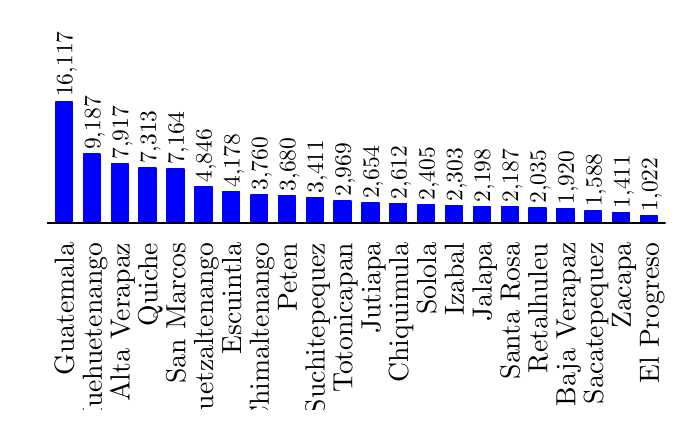
\begin{tikzpicture}[x=1pt,y=1pt]  % Created by tikzDevice version 0.7.0 on 2015-04-16 17:46:46
% !TEX encoding = UTF-8 Unicode
\definecolor[named]{fillColor}{rgb}{1.00,1.00,1.00}
\path[use as bounding box,fill=fillColor,fill opacity=0.00] (0,0) rectangle (230.54,138.04);
\begin{scope}
\path[clip] (  0.00,  0.00) rectangle (230.54,138.04);
\definecolor[named]{drawColor}{rgb}{1.00,1.00,1.00}

\path[draw=drawColor,line width= 0.6pt,line join=round,line cap=round] (  0.00,  0.00) rectangle (230.54,138.04);
\end{scope}
\begin{scope}
\path[clip] (  0.00,  0.00) rectangle (230.54,138.04);

\path[] (  7.11, 67.45) rectangle (230.54,111.19);

\path[] ( 13.15, 67.45) --
	( 13.15,111.19);

\path[] ( 23.22, 67.45) --
	( 23.22,111.19);

\path[] ( 33.28, 67.45) --
	( 33.28,111.19);

\path[] ( 43.34, 67.45) --
	( 43.34,111.19);

\path[] ( 53.41, 67.45) --
	( 53.41,111.19);

\path[] ( 63.47, 67.45) --
	( 63.47,111.19);

\path[] ( 73.54, 67.45) --
	( 73.54,111.19);

\path[] ( 83.60, 67.45) --
	( 83.60,111.19);

\path[] ( 93.67, 67.45) --
	( 93.67,111.19);

\path[] (103.73, 67.45) --
	(103.73,111.19);

\path[] (113.80, 67.45) --
	(113.80,111.19);

\path[] (123.86, 67.45) --
	(123.86,111.19);

\path[] (133.92, 67.45) --
	(133.92,111.19);

\path[] (143.99, 67.45) --
	(143.99,111.19);

\path[] (154.05, 67.45) --
	(154.05,111.19);

\path[] (164.12, 67.45) --
	(164.12,111.19);

\path[] (174.18, 67.45) --
	(174.18,111.19);

\path[] (184.25, 67.45) --
	(184.25,111.19);

\path[] (194.31, 67.45) --
	(194.31,111.19);

\path[] (204.37, 67.45) --
	(204.37,111.19);

\path[] (214.44, 67.45) --
	(214.44,111.19);

\path[] (224.50, 67.45) --
	(224.50,111.19);
\definecolor[named]{drawColor}{rgb}{0.00,0.00,1.00}
\definecolor[named]{fillColor}{rgb}{0.00,0.00,1.00}

\path[draw=drawColor,line width= 0.6pt,line join=round,fill=fillColor] ( 10.13, 67.45) rectangle ( 16.17,111.19);

\path[draw=drawColor,line width= 0.6pt,line join=round,fill=fillColor] ( 20.20, 67.45) rectangle ( 26.24, 92.38);

\path[draw=drawColor,line width= 0.6pt,line join=round,fill=fillColor] ( 30.26, 67.45) rectangle ( 36.30, 88.94);

\path[draw=drawColor,line width= 0.6pt,line join=round,fill=fillColor] ( 40.33, 67.45) rectangle ( 46.36, 87.30);

\path[draw=drawColor,line width= 0.6pt,line join=round,fill=fillColor] ( 50.39, 67.45) rectangle ( 56.43, 86.89);

\path[draw=drawColor,line width= 0.6pt,line join=round,fill=fillColor] ( 60.45, 67.45) rectangle ( 66.49, 80.60);

\path[draw=drawColor,line width= 0.6pt,line join=round,fill=fillColor] ( 70.52, 67.45) rectangle ( 76.56, 78.79);

\path[draw=drawColor,line width= 0.6pt,line join=round,fill=fillColor] ( 80.58, 67.45) rectangle ( 86.62, 77.66);

\path[draw=drawColor,line width= 0.6pt,line join=round,fill=fillColor] ( 90.65, 67.45) rectangle ( 96.69, 77.44);

\path[draw=drawColor,line width= 0.6pt,line join=round,fill=fillColor] (100.71, 67.45) rectangle (106.75, 76.71);

\path[draw=drawColor,line width= 0.6pt,line join=round,fill=fillColor] (110.78, 67.45) rectangle (116.81, 75.51);

\path[draw=drawColor,line width= 0.6pt,line join=round,fill=fillColor] (120.84, 67.45) rectangle (126.88, 74.65);

\path[draw=drawColor,line width= 0.6pt,line join=round,fill=fillColor] (130.90, 67.45) rectangle (136.94, 74.54);

\path[draw=drawColor,line width= 0.6pt,line join=round,fill=fillColor] (140.97, 67.45) rectangle (147.01, 73.98);

\path[draw=drawColor,line width= 0.6pt,line join=round,fill=fillColor] (151.03, 67.45) rectangle (157.07, 73.70);

\path[draw=drawColor,line width= 0.6pt,line join=round,fill=fillColor] (161.10, 67.45) rectangle (167.14, 73.42);

\path[draw=drawColor,line width= 0.6pt,line join=round,fill=fillColor] (171.16, 67.45) rectangle (177.20, 73.39);

\path[draw=drawColor,line width= 0.6pt,line join=round,fill=fillColor] (181.23, 67.45) rectangle (187.26, 72.97);

\path[draw=drawColor,line width= 0.6pt,line join=round,fill=fillColor] (191.29, 67.45) rectangle (197.33, 72.66);

\path[draw=drawColor,line width= 0.6pt,line join=round,fill=fillColor] (201.35, 67.45) rectangle (207.39, 71.76);

\path[draw=drawColor,line width= 0.6pt,line join=round,fill=fillColor] (211.42, 67.45) rectangle (217.46, 71.28);

\path[draw=drawColor,line width= 0.6pt,line join=round,fill=fillColor] (221.48, 67.45) rectangle (227.52, 70.22);
\definecolor[named]{drawColor}{rgb}{0.00,0.00,0.00}
\definecolor[named]{fillColor}{rgb}{0.00,0.00,0.00}

\path[draw=drawColor,line width= 0.6pt,line join=round,fill=fillColor] (  7.11, 67.45) -- (230.54, 67.45);

\node[text=drawColor,rotate= 90.00,anchor=base west,inner sep=0pt, outer sep=0pt, scale=  0.85] at ( 16.19,113.07) {16,117};

\node[text=drawColor,rotate= 90.00,anchor=base west,inner sep=0pt, outer sep=0pt, scale=  0.85] at ( 26.25, 93.92) {9,187};

\node[text=drawColor,rotate= 90.00,anchor=base west,inner sep=0pt, outer sep=0pt, scale=  0.85] at ( 36.32, 90.47) {7,917};

\node[text=drawColor,rotate= 90.00,anchor=base west,inner sep=0pt, outer sep=0pt, scale=  0.85] at ( 46.38, 88.83) {7,313};

\node[text=drawColor,rotate= 90.00,anchor=base west,inner sep=0pt, outer sep=0pt, scale=  0.85] at ( 56.44, 88.43) {7,164};

\node[text=drawColor,rotate= 90.00,anchor=base west,inner sep=0pt, outer sep=0pt, scale=  0.85] at ( 66.51, 82.14) {4,846};

\node[text=drawColor,rotate= 90.00,anchor=base west,inner sep=0pt, outer sep=0pt, scale=  0.85] at ( 76.57, 80.33) {4,178};

\node[text=drawColor,rotate= 90.00,anchor=base west,inner sep=0pt, outer sep=0pt, scale=  0.85] at ( 86.64, 79.19) {3,760};

\node[text=drawColor,rotate= 90.00,anchor=base west,inner sep=0pt, outer sep=0pt, scale=  0.85] at ( 96.70, 78.97) {3,680};

\node[text=drawColor,rotate= 90.00,anchor=base west,inner sep=0pt, outer sep=0pt, scale=  0.85] at (106.77, 78.24) {3,411};

\node[text=drawColor,rotate= 90.00,anchor=base west,inner sep=0pt, outer sep=0pt, scale=  0.85] at (116.83, 77.04) {2,969};

\node[text=drawColor,rotate= 90.00,anchor=base west,inner sep=0pt, outer sep=0pt, scale=  0.85] at (126.89, 76.19) {2,654};

\node[text=drawColor,rotate= 90.00,anchor=base west,inner sep=0pt, outer sep=0pt, scale=  0.85] at (136.96, 76.08) {2,612};

\node[text=drawColor,rotate= 90.00,anchor=base west,inner sep=0pt, outer sep=0pt, scale=  0.85] at (147.02, 75.51) {2,405};

\node[text=drawColor,rotate= 90.00,anchor=base west,inner sep=0pt, outer sep=0pt, scale=  0.85] at (157.09, 75.24) {2,303};

\node[text=drawColor,rotate= 90.00,anchor=base west,inner sep=0pt, outer sep=0pt, scale=  0.85] at (167.15, 74.95) {2,198};

\node[text=drawColor,rotate= 90.00,anchor=base west,inner sep=0pt, outer sep=0pt, scale=  0.85] at (177.22, 74.92) {2,187};

\node[text=drawColor,rotate= 90.00,anchor=base west,inner sep=0pt, outer sep=0pt, scale=  0.85] at (187.28, 74.51) {2,035};

\node[text=drawColor,rotate= 90.00,anchor=base west,inner sep=0pt, outer sep=0pt, scale=  0.85] at (197.35, 74.20) {1,920};

\node[text=drawColor,rotate= 90.00,anchor=base west,inner sep=0pt, outer sep=0pt, scale=  0.85] at (207.41, 73.30) {1,588};

\node[text=drawColor,rotate= 90.00,anchor=base west,inner sep=0pt, outer sep=0pt, scale=  0.85] at (217.47, 72.82) {1,411};

\node[text=drawColor,rotate= 90.00,anchor=base west,inner sep=0pt, outer sep=0pt, scale=  0.85] at (227.54, 71.76) {1,022};
\end{scope}
\begin{scope}
\path[clip] (  0.00,  0.00) rectangle (230.54,138.04);

\path[] (  7.11, 67.45) --
	(  7.11,111.19);
\end{scope}
\begin{scope}
\path[clip] (  0.00,  0.00) rectangle (230.54,138.04);

\path[] (  7.11, 67.45) --
	(230.54, 67.45);
\end{scope}
\begin{scope}
\path[clip] (  0.00,  0.00) rectangle (230.54,138.04);

\path[] ( 13.15, 63.18) --
	( 13.15, 67.45);

\path[] ( 23.22, 63.18) --
	( 23.22, 67.45);

\path[] ( 33.28, 63.18) --
	( 33.28, 67.45);

\path[] ( 43.34, 63.18) --
	( 43.34, 67.45);

\path[] ( 53.41, 63.18) --
	( 53.41, 67.45);

\path[] ( 63.47, 63.18) --
	( 63.47, 67.45);

\path[] ( 73.54, 63.18) --
	( 73.54, 67.45);

\path[] ( 83.60, 63.18) --
	( 83.60, 67.45);

\path[] ( 93.67, 63.18) --
	( 93.67, 67.45);

\path[] (103.73, 63.18) --
	(103.73, 67.45);

\path[] (113.80, 63.18) --
	(113.80, 67.45);

\path[] (123.86, 63.18) --
	(123.86, 67.45);

\path[] (133.92, 63.18) --
	(133.92, 67.45);

\path[] (143.99, 63.18) --
	(143.99, 67.45);

\path[] (154.05, 63.18) --
	(154.05, 67.45);

\path[] (164.12, 63.18) --
	(164.12, 67.45);

\path[] (174.18, 63.18) --
	(174.18, 67.45);

\path[] (184.25, 63.18) --
	(184.25, 67.45);

\path[] (194.31, 63.18) --
	(194.31, 67.45);

\path[] (204.37, 63.18) --
	(204.37, 67.45);

\path[] (214.44, 63.18) --
	(214.44, 67.45);

\path[] (224.50, 63.18) --
	(224.50, 67.45);
\end{scope}
\begin{scope}
\path[clip] (  0.00,  0.00) rectangle (230.54,138.04);
\definecolor[named]{drawColor}{rgb}{0.00,0.00,0.00}

\node[text=drawColor,rotate= 90.00,anchor=base east,inner sep=0pt, outer sep=0pt, scale=  1.00] at ( 16.72, 60.34) {Guatemala};

\node[text=drawColor,rotate= 90.00,anchor=base east,inner sep=0pt, outer sep=0pt, scale=  1.00] at ( 26.79, 60.34) {Huehuetenango};

\node[text=drawColor,rotate= 90.00,anchor=base east,inner sep=0pt, outer sep=0pt, scale=  1.00] at ( 36.85, 60.34) {Alta Verapaz};

\node[text=drawColor,rotate= 90.00,anchor=base east,inner sep=0pt, outer sep=0pt, scale=  1.00] at ( 46.91, 60.34) {Quiche};

\node[text=drawColor,rotate= 90.00,anchor=base east,inner sep=0pt, outer sep=0pt, scale=  1.00] at ( 56.98, 60.34) {San Marcos};

\node[text=drawColor,rotate= 90.00,anchor=base east,inner sep=0pt, outer sep=0pt, scale=  1.00] at ( 67.04, 60.34) {Quetzaltenango};

\node[text=drawColor,rotate= 90.00,anchor=base east,inner sep=0pt, outer sep=0pt, scale=  1.00] at ( 77.11, 60.34) {Escuintla};

\node[text=drawColor,rotate= 90.00,anchor=base east,inner sep=0pt, outer sep=0pt, scale=  1.00] at ( 87.17, 60.34) {Chimaltenango};

\node[text=drawColor,rotate= 90.00,anchor=base east,inner sep=0pt, outer sep=0pt, scale=  1.00] at ( 97.24, 60.34) {Peten};

\node[text=drawColor,rotate= 90.00,anchor=base east,inner sep=0pt, outer sep=0pt, scale=  1.00] at (107.30, 60.34) {Suchitepequez};

\node[text=drawColor,rotate= 90.00,anchor=base east,inner sep=0pt, outer sep=0pt, scale=  1.00] at (117.36, 60.34) {Totonicapan};

\node[text=drawColor,rotate= 90.00,anchor=base east,inner sep=0pt, outer sep=0pt, scale=  1.00] at (127.43, 60.34) {Jutiapa};

\node[text=drawColor,rotate= 90.00,anchor=base east,inner sep=0pt, outer sep=0pt, scale=  1.00] at (137.49, 60.34) {Chiquimula};

\node[text=drawColor,rotate= 90.00,anchor=base east,inner sep=0pt, outer sep=0pt, scale=  1.00] at (147.56, 60.34) {Solola};

\node[text=drawColor,rotate= 90.00,anchor=base east,inner sep=0pt, outer sep=0pt, scale=  1.00] at (157.62, 60.34) {Izabal};

\node[text=drawColor,rotate= 90.00,anchor=base east,inner sep=0pt, outer sep=0pt, scale=  1.00] at (167.69, 60.34) {Jalapa};

\node[text=drawColor,rotate= 90.00,anchor=base east,inner sep=0pt, outer sep=0pt, scale=  1.00] at (177.75, 60.34) {Santa Rosa};

\node[text=drawColor,rotate= 90.00,anchor=base east,inner sep=0pt, outer sep=0pt, scale=  1.00] at (187.81, 60.34) {Retalhuleu};

\node[text=drawColor,rotate= 90.00,anchor=base east,inner sep=0pt, outer sep=0pt, scale=  1.00] at (197.88, 60.34) {Baja Verapaz};

\node[text=drawColor,rotate= 90.00,anchor=base east,inner sep=0pt, outer sep=0pt, scale=  1.00] at (207.94, 60.34) {Sacatepequez};

\node[text=drawColor,rotate= 90.00,anchor=base east,inner sep=0pt, outer sep=0pt, scale=  1.00] at (218.01, 60.34) {Zacapa};

\node[text=drawColor,rotate= 90.00,anchor=base east,inner sep=0pt, outer sep=0pt, scale=  1.00] at (228.07, 60.34) {El Progreso};
\end{scope}
  \end{tikzpicture}}{Instituto Nacional de Estadística, unidad de estadísticas socioculturales.}


\cajita{Faltantes según escolaridad y sexo}{De acuerdo a las distribuciones de las faltas judiciales según el sexo del faltante y el nivel de escolaridad, el 48.1\% de los hombres que cometieron faltas judiciales y el 41.6\% de las mujeres, tenía algún nivel de educación primaria.  
	
	El 12.5\% de los hombre faltantes y el 19.4\% de las mujeres no tenían ninguna formación académica.}{Distribución de las faltas judiciales por sexo, según el nivel educativo del faltante}{República de Guatemala, año 2014, en porcentaje}{\ \\[0mm]\begin{tikzpicture}[x=1pt,y=1pt]  % Created by tikzDevice version 0.10.1 on 2016-02-29 15:08:07
% !TEX encoding = UTF-8 Unicode
\definecolor{fillColor}{RGB}{255,255,255}
\path[use as bounding box,fill=fillColor,fill opacity=0.00] (0,0) rectangle (289.08,198.74);
\begin{scope}
\path[clip] (  0.00,  0.00) rectangle (289.08,198.74);

\path[] (  0.00,  0.00) rectangle (289.08,198.74);
\end{scope}
\begin{scope}
\path[clip] (  0.00,  0.00) rectangle (289.08,198.74);

\path[] (  0.00, 18.46) rectangle (289.08,172.85);

\path[] ( 24.09, 18.46) --
	( 24.09,172.85);

\path[] ( 64.24, 18.46) --
	( 64.24,172.85);

\path[] (104.39, 18.46) --
	(104.39,172.85);

\path[] (144.54, 18.46) --
	(144.54,172.85);

\path[] (184.69, 18.46) --
	(184.69,172.85);

\path[] (224.84, 18.46) --
	(224.84,172.85);

\path[] (264.99, 18.46) --
	(264.99,172.85);
\definecolor{drawColor}{RGB}{0,0,255}
\definecolor{fillColor}{RGB}{0,0,255}

\path[draw=drawColor,line width= 0.6pt,line join=round,fill=fillColor] (  9.54, 18.46) rectangle ( 20.58, 58.48);
\definecolor{drawColor}{RGB}{157,187,255}
\definecolor{fillColor}{RGB}{157,187,255}

\path[draw=drawColor,line width= 0.6pt,line join=round,fill=fillColor] ( 27.60, 18.46) rectangle ( 38.64, 80.76);
\definecolor{drawColor}{RGB}{0,0,255}
\definecolor{fillColor}{RGB}{0,0,255}

\path[draw=drawColor,line width= 0.6pt,line join=round,fill=fillColor] ( 49.69, 18.46) rectangle ( 60.73, 31.42);
\definecolor{drawColor}{RGB}{157,187,255}
\definecolor{fillColor}{RGB}{157,187,255}

\path[draw=drawColor,line width= 0.6pt,line join=round,fill=fillColor] ( 67.75, 18.46) rectangle ( 78.79, 31.04);
\definecolor{drawColor}{RGB}{0,0,255}
\definecolor{fillColor}{RGB}{0,0,255}

\path[draw=drawColor,line width= 0.6pt,line join=round,fill=fillColor] ( 89.84, 18.46) rectangle (100.88,172.85);
\definecolor{drawColor}{RGB}{157,187,255}
\definecolor{fillColor}{RGB}{157,187,255}

\path[draw=drawColor,line width= 0.6pt,line join=round,fill=fillColor] (107.90, 18.46) rectangle (118.94,151.84);
\definecolor{drawColor}{RGB}{0,0,255}
\definecolor{fillColor}{RGB}{0,0,255}

\path[draw=drawColor,line width= 0.6pt,line join=round,fill=fillColor] (129.99, 18.46) rectangle (141.03, 68.35);
\definecolor{drawColor}{RGB}{157,187,255}
\definecolor{fillColor}{RGB}{157,187,255}

\path[draw=drawColor,line width= 0.6pt,line join=round,fill=fillColor] (148.05, 18.46) rectangle (159.09, 50.83);
\definecolor{drawColor}{RGB}{0,0,255}
\definecolor{fillColor}{RGB}{0,0,255}

\path[draw=drawColor,line width= 0.6pt,line join=round,fill=fillColor] (170.14, 18.46) rectangle (181.18, 58.74);
\definecolor{drawColor}{RGB}{157,187,255}
\definecolor{fillColor}{RGB}{157,187,255}

\path[draw=drawColor,line width= 0.6pt,line join=round,fill=fillColor] (188.20, 18.46) rectangle (199.24, 41.57);
\definecolor{drawColor}{RGB}{0,0,255}
\definecolor{fillColor}{RGB}{0,0,255}

\path[draw=drawColor,line width= 0.6pt,line join=round,fill=fillColor] (210.29, 18.46) rectangle (221.33, 23.01);
\definecolor{drawColor}{RGB}{157,187,255}
\definecolor{fillColor}{RGB}{157,187,255}

\path[draw=drawColor,line width= 0.6pt,line join=round,fill=fillColor] (228.35, 18.46) rectangle (239.39, 20.44);
\definecolor{drawColor}{RGB}{0,0,255}
\definecolor{fillColor}{RGB}{0,0,255}

\path[draw=drawColor,line width= 0.6pt,line join=round,fill=fillColor] (250.44, 18.46) rectangle (261.48, 37.19);
\definecolor{drawColor}{RGB}{157,187,255}
\definecolor{fillColor}{RGB}{157,187,255}

\path[draw=drawColor,line width= 0.6pt,line join=round,fill=fillColor] (268.50, 18.46) rectangle (279.54, 73.55);
\definecolor{drawColor}{RGB}{0,0,0}

\path[draw=drawColor,line width= 0.6pt,line join=round] (  0.00, 18.46) -- (289.08, 18.46);

\node[text=drawColor,anchor=base,inner sep=0pt, outer sep=0pt, scale=  0.83] at ( 15.06, 61.72) {12.5};

\node[text=drawColor,anchor=base,inner sep=0pt, outer sep=0pt, scale=  0.83] at ( 33.12, 83.99) {19.4};

\node[text=drawColor,anchor=base,inner sep=0pt, outer sep=0pt, scale=  0.83] at ( 55.21, 34.65) {4.0};

\node[text=drawColor,anchor=base,inner sep=0pt, outer sep=0pt, scale=  0.83] at ( 73.27, 34.28) {3.9};

\node[text=drawColor,anchor=base,inner sep=0pt, outer sep=0pt, scale=  0.83] at ( 95.36,176.08) {48.1};

\node[text=drawColor,anchor=base,inner sep=0pt, outer sep=0pt, scale=  0.83] at (113.42,155.08) {41.6};

\node[text=drawColor,anchor=base,inner sep=0pt, outer sep=0pt, scale=  0.83] at (135.51, 71.58) {15.6};

\node[text=drawColor,anchor=base,inner sep=0pt, outer sep=0pt, scale=  0.83] at (153.57, 54.07) {10.1};

\node[text=drawColor,anchor=base,inner sep=0pt, outer sep=0pt, scale=  0.83] at (175.66, 61.98) {12.6};

\node[text=drawColor,anchor=base,inner sep=0pt, outer sep=0pt, scale=  0.83] at (193.72, 44.81) {7.2};

\node[text=drawColor,anchor=base,inner sep=0pt, outer sep=0pt, scale=  0.83] at (215.81, 26.25) {1.4};

\node[text=drawColor,anchor=base,inner sep=0pt, outer sep=0pt, scale=  0.83] at (233.87, 23.67) {0.6};

\node[text=drawColor,anchor=base,inner sep=0pt, outer sep=0pt, scale=  0.83] at (255.96, 40.42) {5.8};

\node[text=drawColor,anchor=base,inner sep=0pt, outer sep=0pt, scale=  0.83] at (274.02, 76.79) {17.2};

\path[] (  0.00, 18.46) rectangle (289.08,172.85);
\end{scope}
\begin{scope}
\path[clip] (  0.00,  0.00) rectangle (289.08,198.74);

\path[] (  0.00, 18.46) --
	(289.08, 18.46);
\end{scope}
\begin{scope}
\path[clip] (  0.00,  0.00) rectangle (289.08,198.74);

\path[] ( 24.09, 15.71) --
	( 24.09, 18.46);

\path[] ( 64.24, 15.71) --
	( 64.24, 18.46);

\path[] (104.39, 15.71) --
	(104.39, 18.46);

\path[] (144.54, 15.71) --
	(144.54, 18.46);

\path[] (184.69, 15.71) --
	(184.69, 18.46);

\path[] (224.84, 15.71) --
	(224.84, 18.46);

\path[] (264.99, 15.71) --
	(264.99, 18.46);
\end{scope}
\begin{scope}
\path[clip] (  0.00,  0.00) rectangle (289.08,198.74);
\definecolor{drawColor}{RGB}{0,0,0}

\node[text=drawColor,anchor=base,inner sep=0pt, outer sep=0pt, scale=  1.00] at ( 24.09,  5.69) {Ninguno};

\node[text=drawColor,anchor=base,inner sep=0pt, outer sep=0pt, scale=  1.00] at ( 64.24,  5.69) {Preprimaria};

\node[text=drawColor,anchor=base,inner sep=0pt, outer sep=0pt, scale=  1.00] at (104.39,  5.69) {Primaria};

\node[text=drawColor,anchor=base,inner sep=0pt, outer sep=0pt, scale=  1.00] at (144.54,  5.69) {Básicos};

\node[text=drawColor,anchor=base,inner sep=0pt, outer sep=0pt, scale=  1.00] at (184.69,  5.69) {Diversificado};

\node[text=drawColor,anchor=base,inner sep=0pt, outer sep=0pt, scale=  1.00] at (224.84,  5.69) {Superior};

\node[text=drawColor,anchor=base,inner sep=0pt, outer sep=0pt, scale=  1.00] at (264.99,  5.69) {Ignorado};
\end{scope}
\begin{scope}
\path[clip] (  0.00,  0.00) rectangle (289.08,198.74);
\coordinate (apoyo) at (55.98,189.21);
\coordinate (longitudFicticia) at (7.11,9.53);
\coordinate (longitud) at (7.11,7.11);
\coordinate (desX) at (142.21,0);
\coordinate (desY) at (0,1.21);
\definecolor[named]{ct1}{HTML}{
0000FF
}
\definecolor[named]{ct2}{HTML}{
9DBBFF
}
\definecolor[named]{ctb1}{HTML}{
0000FF
}
\definecolor[named]{ctb2}{HTML}{
9DBBFF
}
\path [fill=none] (apoyo) rectangle ($(apoyo)+(longitudFicticia)$)
node [xshift=0.3cm,inner sep=0pt, outer sep=0pt,midway,right,scale = 0.9]{Hombre};
\draw [color = ctb1,fill=ct1] ( $(apoyo)  + (desY) $) rectangle ($(apoyo)+ (desY) +(longitud)$);
\path [fill=none] ($(apoyo)+(desX)$) rectangle ($(apoyo)+(desX)+(longitudFicticia)$)
node [xshift=0.3cm,inner sep=0pt, outer sep=0pt,midway,right,scale = 0.9]{Mujer};
\draw [color = ctb2 ,fill=ct2] ( $(apoyo)  + (desY) + (desX) $) rectangle ($(apoyo)+ (desY)+ (desX) +(longitud)$);
\end{scope}
  \end{tikzpicture}}{Instituto Nacional de Estadística, unidad de estadísticas socioculturales.}


\cajita{Faltantes con educación primaria y tipo de falta}{En relación al tipo de falta se observa que en general más del 50\% de los tipos de faltas son cometidos por personas con estudios hasta primaria.}{Proporción de los faltantes que tienen hasta educación primaria, según tipo de falta\textollamada{Se encluyen: sin escolaridad, preprimaria y primaria.}}{República de Guatemala, año 2014, en porcentaje}{\ \\[0mm]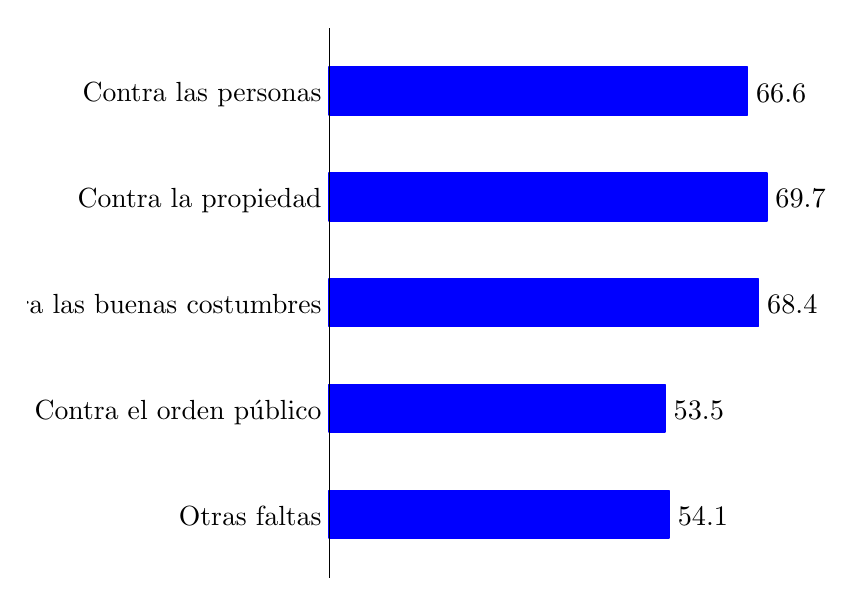
\begin{tikzpicture}[x=1pt,y=1pt]  % Created by tikzDevice version 0.10.1 on 2016-02-29 15:09:30
% !TEX encoding = UTF-8 Unicode
\definecolor{fillColor}{RGB}{255,255,255}
\path[use as bounding box,fill=fillColor,fill opacity=0.00] (0,0) rectangle (289.08,198.74);
\begin{scope}
\path[clip] (  0.00,  0.00) rectangle (289.08,198.74);

\path[] (  0.00,  0.00) rectangle (289.08,198.74);
\end{scope}
\begin{scope}
\path[clip] (  0.00,  0.00) rectangle (289.08,198.74);

\path[] (108.92,  0.00) rectangle (267.09,198.74);

\path[] (108.92, 22.93) --
	(267.09, 22.93);

\path[] (108.92, 61.15) --
	(267.09, 61.15);

\path[] (108.92, 99.37) --
	(267.09, 99.37);

\path[] (108.92,137.59) --
	(267.09,137.59);

\path[] (108.92,175.81) --
	(267.09,175.81);
\definecolor{drawColor}{RGB}{0,0,255}
\definecolor{fillColor}{RGB}{0,0,255}

\path[draw=drawColor,line width= 0.6pt,line join=round,fill=fillColor] (108.92, 14.33) rectangle (231.79, 31.53);

\path[draw=drawColor,line width= 0.6pt,line join=round,fill=fillColor] (108.92, 52.55) rectangle (230.32, 69.75);

\path[draw=drawColor,line width= 0.6pt,line join=round,fill=fillColor] (108.92, 90.77) rectangle (264.11,107.97);

\path[draw=drawColor,line width= 0.6pt,line join=round,fill=fillColor] (108.92,128.99) rectangle (267.09,146.19);

\path[draw=drawColor,line width= 0.6pt,line join=round,fill=fillColor] (108.92,167.21) rectangle (260.10,184.41);
\definecolor{drawColor}{RGB}{0,0,0}

\path[draw=drawColor,line width= 0.1pt,line join=round] (108.92,  0.00) -- (108.92,198.74);

\node[text=drawColor,anchor=base west,inner sep=0pt, outer sep=0pt, scale=  1.02] at (234.92, 18.96) {54.1};

\node[text=drawColor,anchor=base west,inner sep=0pt, outer sep=0pt, scale=  1.02] at (233.45, 57.18) {53.5};

\node[text=drawColor,anchor=base west,inner sep=0pt, outer sep=0pt, scale=  1.02] at (267.24, 95.40) {68.4};

\node[text=drawColor,anchor=base west,inner sep=0pt, outer sep=0pt, scale=  1.02] at (270.21,133.62) {69.7};

\node[text=drawColor,anchor=base west,inner sep=0pt, outer sep=0pt, scale=  1.02] at (263.23,171.84) {66.6};

\path[] (108.92,  0.00) rectangle (267.09,198.74);
\end{scope}
\begin{scope}
\path[clip] (  0.00,  0.00) rectangle (289.08,198.74);

\path[] (108.92,  0.00) --
	(108.92,198.74);
\end{scope}
\begin{scope}
\path[clip] (  0.00,  0.00) rectangle (289.08,198.74);
\definecolor{drawColor}{RGB}{0,0,0}

\node[text=drawColor,anchor=base east,inner sep=0pt, outer sep=0pt, scale=  1.00] at (106.17, 19.02) {Otras faltas};

\node[text=drawColor,anchor=base east,inner sep=0pt, outer sep=0pt, scale=  1.00] at (106.17, 57.24) {Contra el orden público};

\node[text=drawColor,anchor=base east,inner sep=0pt, outer sep=0pt, scale=  1.00] at (106.17, 95.46) {Contra las buenas costumbres};

\node[text=drawColor,anchor=base east,inner sep=0pt, outer sep=0pt, scale=  1.00] at (106.17,133.68) {Contra la propiedad};

\node[text=drawColor,anchor=base east,inner sep=0pt, outer sep=0pt, scale=  1.00] at (106.17,171.90) {Contra las personas};
\end{scope}
\begin{scope}
\path[clip] (  0.00,  0.00) rectangle (289.08,198.74);

\path[] (106.17, 22.93) --
	(108.92, 22.93);

\path[] (106.17, 61.15) --
	(108.92, 61.15);

\path[] (106.17, 99.37) --
	(108.92, 99.37);

\path[] (106.17,137.59) --
	(108.92,137.59);

\path[] (106.17,175.81) --
	(108.92,175.81);
\end{scope}
  \end{tikzpicture}}{Instituto Nacional de Estadística, unidad de estadísticas socioculturales.}


\cajita{Faltantes con educación primaria y edad}{Al separar a los faltantes por grupos de edad y calcular la proporción de los que tienen hasta algún estudio del nivel primario, se observa en los grupos de edad que más del 50\% de las faltas cometidas es por personas con ese nivel educativo.}{Proporción de los faltantes que tienen hasta educación primaria, según rangos de edad\textollamada{Se encluyen: sin escolaridad, preprimaria y primaria.}}{República de Guatemala, año 2014, en porcentaje}{\ \\[0mm]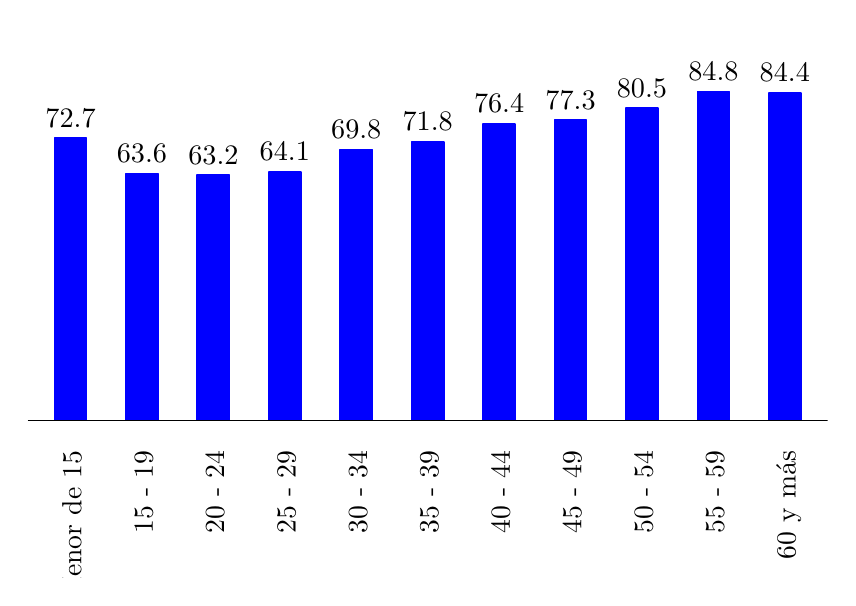
\begin{tikzpicture}[x=1pt,y=1pt]  % Created by tikzDevice version 0.10.1 on 2016-02-29 15:10:19
% !TEX encoding = UTF-8 Unicode
\definecolor{fillColor}{RGB}{255,255,255}
\path[use as bounding box,fill=fillColor,fill opacity=0.00] (0,0) rectangle (289.08,198.74);
\begin{scope}
\path[clip] (  0.00,  0.00) rectangle (289.08,198.74);

\path[] (  0.00,  0.00) rectangle (289.08,198.74);
\end{scope}
\begin{scope}
\path[clip] (  0.00,  0.00) rectangle (289.08,198.74);

\path[] (  0.00, 50.83) rectangle (289.08,181.67);

\path[] ( 15.49, 50.83) --
	( 15.49,181.67);

\path[] ( 41.30, 50.83) --
	( 41.30,181.67);

\path[] ( 67.11, 50.83) --
	( 67.11,181.67);

\path[] ( 92.92, 50.83) --
	( 92.92,181.67);

\path[] (118.73, 50.83) --
	(118.73,181.67);

\path[] (144.54, 50.83) --
	(144.54,181.67);

\path[] (170.35, 50.83) --
	(170.35,181.67);

\path[] (196.16, 50.83) --
	(196.16,181.67);

\path[] (221.97, 50.83) --
	(221.97,181.67);

\path[] (247.78, 50.83) --
	(247.78,181.67);

\path[] (273.59, 50.83) --
	(273.59,181.67);
\definecolor{drawColor}{RGB}{0,0,255}
\definecolor{fillColor}{RGB}{0,0,255}

\path[draw=drawColor,line width= 0.6pt,line join=round,fill=fillColor] (  9.68, 56.78) rectangle ( 21.29,158.81);

\path[draw=drawColor,line width= 0.6pt,line join=round,fill=fillColor] ( 35.49, 56.78) rectangle ( 47.10,146.01);

\path[draw=drawColor,line width= 0.6pt,line join=round,fill=fillColor] ( 61.30, 56.78) rectangle ( 72.92,145.45);

\path[draw=drawColor,line width= 0.6pt,line join=round,fill=fillColor] ( 87.11, 56.78) rectangle ( 98.73,146.69);

\path[draw=drawColor,line width= 0.6pt,line join=round,fill=fillColor] (112.92, 56.78) rectangle (124.54,154.71);

\path[draw=drawColor,line width= 0.6pt,line join=round,fill=fillColor] (138.73, 56.78) rectangle (150.35,157.49);

\path[draw=drawColor,line width= 0.6pt,line join=round,fill=fillColor] (164.54, 56.78) rectangle (176.16,163.94);

\path[draw=drawColor,line width= 0.6pt,line join=round,fill=fillColor] (190.35, 56.78) rectangle (201.97,165.28);

\path[draw=drawColor,line width= 0.6pt,line join=round,fill=fillColor] (216.16, 56.78) rectangle (227.78,169.66);

\path[draw=drawColor,line width= 0.6pt,line join=round,fill=fillColor] (241.98, 56.78) rectangle (253.59,175.72);

\path[draw=drawColor,line width= 0.6pt,line join=round,fill=fillColor] (267.79, 56.78) rectangle (279.40,175.25);
\definecolor{drawColor}{RGB}{0,0,0}

\path[draw=drawColor,line width= 0.1pt,line join=round] (  0.00, 56.78) -- (289.08, 56.78);

\node[text=drawColor,anchor=base,inner sep=0pt, outer sep=0pt, scale=  1.02] at ( 15.49,162.78) {72.7};

\node[text=drawColor,anchor=base,inner sep=0pt, outer sep=0pt, scale=  1.02] at ( 41.30,149.98) {63.6};

\node[text=drawColor,anchor=base,inner sep=0pt, outer sep=0pt, scale=  1.02] at ( 67.11,149.42) {63.2};

\node[text=drawColor,anchor=base,inner sep=0pt, outer sep=0pt, scale=  1.02] at ( 92.92,150.66) {64.1};

\node[text=drawColor,anchor=base,inner sep=0pt, outer sep=0pt, scale=  1.02] at (118.73,158.68) {69.8};

\node[text=drawColor,anchor=base,inner sep=0pt, outer sep=0pt, scale=  1.02] at (144.54,161.46) {71.8};

\node[text=drawColor,anchor=base,inner sep=0pt, outer sep=0pt, scale=  1.02] at (170.35,167.91) {76.4};

\node[text=drawColor,anchor=base,inner sep=0pt, outer sep=0pt, scale=  1.02] at (196.16,169.25) {77.3};

\node[text=drawColor,anchor=base,inner sep=0pt, outer sep=0pt, scale=  1.02] at (221.97,173.63) {80.5};

\node[text=drawColor,anchor=base,inner sep=0pt, outer sep=0pt, scale=  1.02] at (247.78,179.69) {84.8};

\node[text=drawColor,anchor=base,inner sep=0pt, outer sep=0pt, scale=  1.02] at (273.59,179.22) {84.4};

\path[] (  0.00, 50.83) rectangle (289.08,181.67);
\end{scope}
\begin{scope}
\path[clip] (  0.00,  0.00) rectangle (289.08,198.74);

\path[] (  0.00, 50.83) --
	(289.08, 50.83);
\end{scope}
\begin{scope}
\path[clip] (  0.00,  0.00) rectangle (289.08,198.74);

\path[] ( 15.49, 48.08) --
	( 15.49, 50.83);

\path[] ( 41.30, 48.08) --
	( 41.30, 50.83);

\path[] ( 67.11, 48.08) --
	( 67.11, 50.83);

\path[] ( 92.92, 48.08) --
	( 92.92, 50.83);

\path[] (118.73, 48.08) --
	(118.73, 50.83);

\path[] (144.54, 48.08) --
	(144.54, 50.83);

\path[] (170.35, 48.08) --
	(170.35, 50.83);

\path[] (196.16, 48.08) --
	(196.16, 50.83);

\path[] (221.97, 48.08) --
	(221.97, 50.83);

\path[] (247.78, 48.08) --
	(247.78, 50.83);

\path[] (273.59, 48.08) --
	(273.59, 50.83);
\end{scope}
\begin{scope}
\path[clip] (  0.00,  0.00) rectangle (289.08,198.74);
\definecolor{drawColor}{RGB}{0,0,0}

\node[text=drawColor,rotate= 90.00,anchor=base east,inner sep=0pt, outer sep=0pt, scale=  1.00] at ( 19.39, 45.88) {Menor de 15};

\node[text=drawColor,rotate= 90.00,anchor=base east,inner sep=0pt, outer sep=0pt, scale=  1.00] at ( 45.21, 45.88) {15 - 19};

\node[text=drawColor,rotate= 90.00,anchor=base east,inner sep=0pt, outer sep=0pt, scale=  1.00] at ( 71.02, 45.88) {20 - 24};

\node[text=drawColor,rotate= 90.00,anchor=base east,inner sep=0pt, outer sep=0pt, scale=  1.00] at ( 96.83, 45.88) {25 - 29};

\node[text=drawColor,rotate= 90.00,anchor=base east,inner sep=0pt, outer sep=0pt, scale=  1.00] at (122.64, 45.88) {30 - 34};

\node[text=drawColor,rotate= 90.00,anchor=base east,inner sep=0pt, outer sep=0pt, scale=  1.00] at (148.45, 45.88) {35 - 39};

\node[text=drawColor,rotate= 90.00,anchor=base east,inner sep=0pt, outer sep=0pt, scale=  1.00] at (174.26, 45.88) {40 - 44};

\node[text=drawColor,rotate= 90.00,anchor=base east,inner sep=0pt, outer sep=0pt, scale=  1.00] at (200.07, 45.88) {45 - 49};

\node[text=drawColor,rotate= 90.00,anchor=base east,inner sep=0pt, outer sep=0pt, scale=  1.00] at (225.88, 45.88) {50 - 54};

\node[text=drawColor,rotate= 90.00,anchor=base east,inner sep=0pt, outer sep=0pt, scale=  1.00] at (251.69, 45.88) {55 - 59};

\node[text=drawColor,rotate= 90.00,anchor=base east,inner sep=0pt, outer sep=0pt, scale=  1.00] at (277.50, 45.88) {60 y más};
\end{scope}
  \end{tikzpicture}}{Instituto Nacional de Estadística, unidad de estadísticas socioculturales.}



\cajita{Faltantes según escolaridad y etnicidad}{En cuanto a la etnicidad y la escolaridad, eran de etnia indígena: el 52.5\% de los faltantes sin ninguna formación escolar, el 43.9\% de los que tenían algún grado de primaria, siendo los dos grupos mayores.
	
	En cuanto a las faltas cometidas por personas con nivel superior de escolaridad, el 26.5\% eran personas indígenas y el 73.5\% eran no indígenas. }{Proporción de los faltantes de etnia indígena, según nivel de escolaridad}{República de Guatemala, año 2014, en porcentaje}{\ \\[0mm]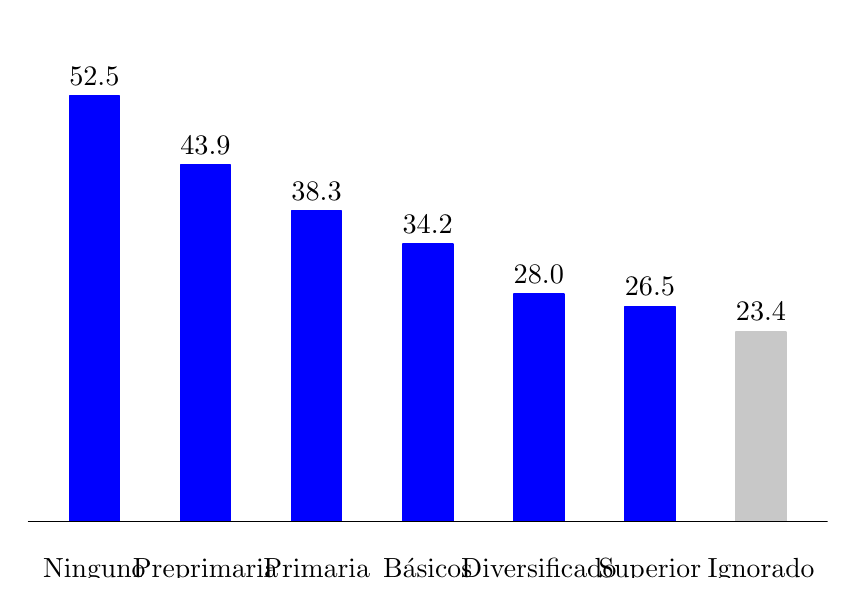
\begin{tikzpicture}[x=1pt,y=1pt]  % Created by tikzDevice version 0.10.1 on 2016-02-29 15:11:16
% !TEX encoding = UTF-8 Unicode
\definecolor{fillColor}{RGB}{255,255,255}
\path[use as bounding box,fill=fillColor,fill opacity=0.00] (0,0) rectangle (289.08,198.74);
\begin{scope}
\path[clip] (  0.00,  0.00) rectangle (289.08,198.74);

\path[] (  0.00,  0.00) rectangle (289.08,198.74);
\end{scope}
\begin{scope}
\path[clip] (  0.00,  0.00) rectangle (289.08,198.74);

\path[] (  0.00, 12.77) rectangle (289.08,181.67);

\path[] ( 24.09, 12.77) --
	( 24.09,181.67);

\path[] ( 64.24, 12.77) --
	( 64.24,181.67);

\path[] (104.39, 12.77) --
	(104.39,181.67);

\path[] (144.54, 12.77) --
	(144.54,181.67);

\path[] (184.69, 12.77) --
	(184.69,181.67);

\path[] (224.84, 12.77) --
	(224.84,181.67);

\path[] (264.99, 12.77) --
	(264.99,181.67);
\definecolor{drawColor}{RGB}{0,0,255}
\definecolor{fillColor}{RGB}{0,0,255}

\path[draw=drawColor,line width= 0.6pt,line join=round,fill=fillColor] ( 15.06, 20.44) rectangle ( 33.12,173.99);

\path[draw=drawColor,line width= 0.6pt,line join=round,fill=fillColor] ( 55.21, 20.44) rectangle ( 73.27,149.00);

\path[draw=drawColor,line width= 0.6pt,line join=round,fill=fillColor] ( 95.36, 20.44) rectangle (113.42,132.49);

\path[draw=drawColor,line width= 0.6pt,line join=round,fill=fillColor] (135.51, 20.44) rectangle (153.57,120.57);

\path[draw=drawColor,line width= 0.6pt,line join=round,fill=fillColor] (175.66, 20.44) rectangle (193.72,102.41);

\path[draw=drawColor,line width= 0.6pt,line join=round,fill=fillColor] (215.81, 20.44) rectangle (233.87, 97.97);
\definecolor{drawColor}{RGB}{200,200,200}
\definecolor{fillColor}{RGB}{200,200,200}

\path[draw=drawColor,line width= 0.6pt,line join=round,fill=fillColor] (255.96, 20.44) rectangle (274.02, 88.86);
\definecolor{drawColor}{RGB}{0,0,0}

\path[draw=drawColor,line width= 0.1pt,line join=round] (  0.00, 20.44) -- (289.08, 20.44);

\node[text=drawColor,anchor=base,inner sep=0pt, outer sep=0pt, scale=  1.02] at ( 24.09,177.96) {52.5};

\node[text=drawColor,anchor=base,inner sep=0pt, outer sep=0pt, scale=  1.02] at ( 64.24,152.97) {43.9};

\node[text=drawColor,anchor=base,inner sep=0pt, outer sep=0pt, scale=  1.02] at (104.39,136.47) {38.3};

\node[text=drawColor,anchor=base,inner sep=0pt, outer sep=0pt, scale=  1.02] at (144.54,124.54) {34.2};

\node[text=drawColor,anchor=base,inner sep=0pt, outer sep=0pt, scale=  1.02] at (184.69,106.38) {28.0};

\node[text=drawColor,anchor=base,inner sep=0pt, outer sep=0pt, scale=  1.02] at (224.84,101.94) {26.5};

\node[text=drawColor,anchor=base,inner sep=0pt, outer sep=0pt, scale=  1.02] at (264.99, 92.83) {23.4};

\path[] (  0.00, 12.77) rectangle (289.08,181.67);
\end{scope}
\begin{scope}
\path[clip] (  0.00,  0.00) rectangle (289.08,198.74);

\path[] (  0.00, 12.77) --
	(289.08, 12.77);
\end{scope}
\begin{scope}
\path[clip] (  0.00,  0.00) rectangle (289.08,198.74);

\path[] ( 24.09, 10.02) --
	( 24.09, 12.77);

\path[] ( 64.24, 10.02) --
	( 64.24, 12.77);

\path[] (104.39, 10.02) --
	(104.39, 12.77);

\path[] (144.54, 10.02) --
	(144.54, 12.77);

\path[] (184.69, 10.02) --
	(184.69, 12.77);

\path[] (224.84, 10.02) --
	(224.84, 12.77);

\path[] (264.99, 10.02) --
	(264.99, 12.77);
\end{scope}
\begin{scope}
\path[clip] (  0.00,  0.00) rectangle (289.08,198.74);
\definecolor{drawColor}{RGB}{0,0,0}

\node[text=drawColor,anchor=base,inner sep=0pt, outer sep=0pt, scale=  1.00] at ( 24.09, -0.00) {Ninguno};

\node[text=drawColor,anchor=base,inner sep=0pt, outer sep=0pt, scale=  1.00] at ( 64.24, -0.00) {Preprimaria};

\node[text=drawColor,anchor=base,inner sep=0pt, outer sep=0pt, scale=  1.00] at (104.39, -0.00) {Primaria};

\node[text=drawColor,anchor=base,inner sep=0pt, outer sep=0pt, scale=  1.00] at (144.54, -0.00) {Básicos};

\node[text=drawColor,anchor=base,inner sep=0pt, outer sep=0pt, scale=  1.00] at (184.69, -0.00) {Diversificado};

\node[text=drawColor,anchor=base,inner sep=0pt, outer sep=0pt, scale=  1.00] at (224.84, -0.00) {Superior};

\node[text=drawColor,anchor=base,inner sep=0pt, outer sep=0pt, scale=  1.00] at (264.99, -0.00) {Ignorado};
\end{scope}
  \end{tikzpicture}}{Instituto Nacional de Estadística, unidad de estadísticas socioculturales.}



\cajita{Faltantes según escolaridad y área de residencia}{De acuerdo al área de residencia según el nivel de escolaridad del faltante, el 44.6\% de los faltantes sin ningún nivel educativo residían en el área urbana, y el 55.4\% en el área rural.
	
	En las categorías restantes, más del 50\% de los faltantes en cada nivel educativo residía en el área urbana.  }{Proporción de los faltantes que residen en el área urbana, según nivel de escolaridad}{República de Guatemala, año 2014, en porcentaje}{\ \\[0mm]\begin{tikzpicture}[x=1pt,y=1pt]  % Created by tikzDevice version 0.10.1 on 2016-02-29 14:40:32
% !TEX encoding = UTF-8 Unicode
\definecolor{fillColor}{RGB}{255,255,255}
\path[use as bounding box,fill=fillColor,fill opacity=0.00] (0,0) rectangle (289.08,198.74);
\begin{scope}
\path[clip] (  0.00,  0.00) rectangle (289.08,198.74);

\path[] (  0.00,  0.00) rectangle (289.08,198.74);
\end{scope}
\begin{scope}
\path[clip] (  0.00,  0.00) rectangle (289.08,198.74);

\path[] ( -4.90, 15.61) rectangle (280.54,191.48);

\path[] (  0.00, 52.34) --
	(280.54, 52.34);

\path[] (  0.00,109.79) --
	(280.54,109.79);

\path[] (  0.00,167.25) --
	(280.54,167.25);

\path[] (  0.00, 23.61) --
	(280.54, 23.61);

\path[] (  0.00, 81.06) --
	(280.54, 81.06);

\path[] (  0.00,138.52) --
	(280.54,138.52);

\path[] ( 28.04, 15.61) --
	( 28.04,191.48);

\path[] ( 82.93, 15.61) --
	( 82.93,191.48);

\path[] (137.82, 15.61) --
	(137.82,191.48);

\path[] (192.72, 15.61) --
	(192.72,191.48);

\path[] (247.61, 15.61) --
	(247.61,191.48);
\definecolor{drawColor}{RGB}{0,0,255}

\path[draw=drawColor,line width= 1.7pt,line join=round] ( 28.04,182.08) --
	( 82.93,179.87) --
	(137.82,183.49) --
	(192.72,178.74) --
	(247.61,175.17);
\definecolor{drawColor}{RGB}{0,0,0}

\node[text=drawColor,anchor=base,inner sep=0pt, outer sep=0pt, scale=  1.02] at ( 28.04,186.05) {3.8};

\node[text=drawColor,anchor=base,inner sep=0pt, outer sep=0pt, scale=  1.02] at ( 82.93,167.95) {3.7};

\node[text=drawColor,anchor=base,inner sep=0pt, outer sep=0pt, scale=  1.02] at (137.82,187.46) {3.8};

\node[text=drawColor,anchor=base west,inner sep=0pt, outer sep=0pt, scale=  1.02] at (192.72,182.71) {3.7};

\node[text=drawColor,anchor=base,inner sep=0pt, outer sep=0pt, scale=  1.02] at (247.61,163.26) {3.6};

\path[draw=drawColor,line width= 0.1pt,line join=round] (  0.00, 23.61) -- (280.54, 23.61);

\path[] ( -4.90, 15.61) rectangle (280.54,191.48);
\end{scope}
\begin{scope}
\path[clip] (  0.00,  0.00) rectangle (289.08,198.74);

\path[] (  0.00, 15.61) --
	(280.54, 15.61);
\end{scope}
\begin{scope}
\path[clip] (  0.00,  0.00) rectangle (289.08,198.74);

\path[] ( 28.04, 12.86) --
	( 28.04, 15.61);

\path[] ( 82.93, 12.86) --
	( 82.93, 15.61);

\path[] (137.82, 12.86) --
	(137.82, 15.61);

\path[] (192.72, 12.86) --
	(192.72, 15.61);

\path[] (247.61, 12.86) --
	(247.61, 15.61);
\end{scope}
\begin{scope}
\path[clip] (  0.00,  0.00) rectangle (289.08,198.74);
\definecolor{drawColor}{RGB}{0,0,0}

\node[text=drawColor,anchor=base,inner sep=0pt, outer sep=0pt, scale=  1.00] at ( 28.04,  2.85) {2010};

\node[text=drawColor,anchor=base,inner sep=0pt, outer sep=0pt, scale=  1.00] at ( 82.93,  2.85) {2011};

\node[text=drawColor,anchor=base,inner sep=0pt, outer sep=0pt, scale=  1.00] at (137.82,  2.85) {2012};

\node[text=drawColor,anchor=base,inner sep=0pt, outer sep=0pt, scale=  1.00] at (192.72,  2.85) {2013};

\node[text=drawColor,anchor=base,inner sep=0pt, outer sep=0pt, scale=  1.00] at (247.61,  2.85) {2014};
\end{scope}
  \end{tikzpicture}}{Instituto Nacional de Estadística, unidad de estadísticas socioculturales.}


